\documentclass[10pt]{article}
\usepackage{amsmath}
\usepackage{amsfonts}
\usepackage{graphicx}
%\usepackage{epstopdf}
\usepackage{hyperref}
\usepackage[left=.9in,right=.9in,top=.7in,bottom=.7in]{geometry}
%\usepackage[left=1.1in,right=1.1in,top=.7in,bottom=.7in]{geometry}
\usepackage{multirow}
\usepackage{verbatim}
\usepackage{fancyhdr}
\usepackage[small,compact]{titlesec} 
\usepackage{color}
\usepackage{ulem}
\usepackage{natbib}
\renewcommand{\cite}{\citet}

%\usepackage[screen,nopanel,gray]{pdfscreen}
%\screensize{4in}{5.33in}
%\margins{0.75in}{0.75in}{0.75in}{0.75in}


%\usepackage{pxfonts}
%\usepackage{isomath}
\usepackage{mathpazo}
%\usepackage{arev} %     (Arev/Vera Sans)
%\usepackage{eulervm} %_   (Euler Math)
%\usepackage{fixmath} %  (Computer Modern)
%\usepackage{hvmath} %_   (HV-Math/Helvetica)
%\usepackage{tmmath} %_   (TM-Math/Times)
%\usepackage{cmbright}
%\usepackage{ccfonts} \usepackage[T1]{fontenc}
%\usepackage[garamond]{mathdesign}

\newcommand{\argmax}{\operatornamewithlimits{arg\,max}}
\newcommand{\argmin}{\operatornamewithlimits{arg\,min}}
\newcommand{\myTable}[1]{\begin{table}[b]\caption{#1}
    \begin{minipage}{\linewidth} \begin{center}}
\newcommand{\myTableEnd}{\end{center}\end{minipage}\end{table}}

\def\inprobLOW{\rightarrow_p}
\def\inprobHIGH{\,{\buildrel p \over \rightarrow}\,} 
\def\inprob{\,{\inprobHIGH}\,} 
\def\indist{\,{\buildrel d \over \rightarrow}\,} 

\newtheorem{theorem}{Theorem}

%\pagestyle{fancy}
\renewcommand{\sectionmark}[1]{\markright{#1}{}}
 
%\fancyhead[LE,LO]{\thepage}
%\fancyhead[CE,CO]{\rightmark}
%\fancyfoot[C]{}

\title{Economics 526 - Mathematics for Economists}
\date{Term 1, 2014}
\author{Paul Schrimpf}

\makeatletter
\renewcommand{\@maketitle}{
  \null
  \begin{center}%
    {\large \textbf{\@title} \par \normalsize \@date \par \@author}%
  \end{center}%
  \par} 
\makeatother

\begin{document}

\maketitle

This is a course of mathematics for students in our Economics MA
program. It covers powerful mathematical tools that often appear
in the modern economic literature. It is essential for the students'
success in other courses to master the materials taught in this
course.

Yawen Liang (neway.liang@gmail.com) and Zhengfei Yu
(yuzhengfei@gmail.com) are the course TA's.  Lecture notes are posted
at \url{http://faculty.arts.ubc.ca/pschrimpf/526/526.html}. Currently
these notes are from last year. The notes will be updated throughout
the term. Problem sets, solutions, and grades will be posted on the
course's \url{https://connect.ubc.ca} page.

 My email is
\href{mailto:schrimp@mail.ubc.ca}{schrimpf@mail.ubc.ca}, and my office
phone number is 604-822-5360. There is a discussion board on the
course's \url{https://connect.ubc.ca} page. I will answer questions on
that as well. I encourage you to use it whenever possible so that
all students can see the questions and answers.

\section{Schedule}
\begin{tabular}{l c c l}
  \hline 
  & \textbf{Day(s)} & \textbf{Time} & \textbf{Location} \\
  Lecture & Monday \& Wednesday & 11:00am-1:00pm &
  \href{https://ssc.adm.ubc.ca/classroomservices/function/viewlocation?userEvent=ShowLocation&buildingID=GEOG&roomID=101}{Geography
  101} \\
  Tutorial & Monday & 8:30am-10:00am &
  \href{https://ssc.adm.ubc.ca/classroomservices/function/viewlocation?userEvent=ShowLocation&buildingID=BRKX&roomID=2365}
  {Brock Hall Annex 2365}  \\
  Office hours \\
  \; Paul & Wednesday & 5:00pm-6:00pm & Buchanan Tower 926 \\
  \; Yawen & TBA & & \\ 
  \; Zhengfei & TBA & & \\ \hline
  Exams \\
  \; Midterm & Monday, October 6th & 11:00am-1:00pm & \href{https://ssc.adm.ubc.ca/classroomservices/function/viewlocation?userEvent=ShowLocation&buildingID=GEOG&roomID=101}{Geography
  101} \\
  \; Final & Wednesday, November 12th & 11:00am-1:00pm & \href{https://ssc.adm.ubc.ca/classroomservices/function/viewlocation?userEvent=ShowLocation&buildingID=GEOG&roomID=101}{Geography
  101} \\
  No class \\
  \; Thanksgiving & Monday, October 13th \\
  \\ \hline 
\end{tabular} \\
Office hours are subject to change. Any changes in office hours will
be posted on the course web page. If you cannot come to my office
hours, feel free to drop by anytime or email me to schedule an
appointment.  

\section{Course Work}

The course work will consist of a series of problem sets and two
exams. 

\subsection{Problem Sets}
Problem sets will be due approximately weekly.  Students should solve
each problem set and turn in their work by the specified due
date. Also, students should study the solution to each problem set
carefully, regardless of their performances in the problem
set. Students may work together on problem sets, but each student
should write their own solutions. 

\subsection{Exams}
Two in-class exams will be given on October 6th and November 12th. If
a student misses the first exam due to an objectively verifiable,
unavoidable emergency situation, the student's grade will be
determined by setting his or her first exam's grade equal to his or her
second exam's grade. If a student misses the first exam for any other
reasons, the student receives zero points for the first exam.

\subsection{Grading}
The course grade weights the problem sets by 0.15, the First exam by
0.40 and the second exam by 0.45. If a student finds an error in the
grading of a problem set or exam, the student should contact the
teaching assistants (for problem sets) or me (for an exam) within one
week of the day the graded problem sets or exams were made
available. We will then regrade the entire problem set or exam, and
your total score may increase or decrease as a result.  The
distribution of grades in this course for the past seven years is shown
below.
\href{http://www.arts.ubc.ca/faculty-amp-staff/resources/courses-and-grading/grading-guidelines.html}
{The Faculty of Arts grading guidelines} recommend that 5-25\% of the
class receive A's (80-100) and not more than 75\% receive A's or B's
(68-79). Grades may be scaled up to meet these guidelines and/or match
the historical distribution of grades, but they will not be scaled
down. 

\begin{centering}
  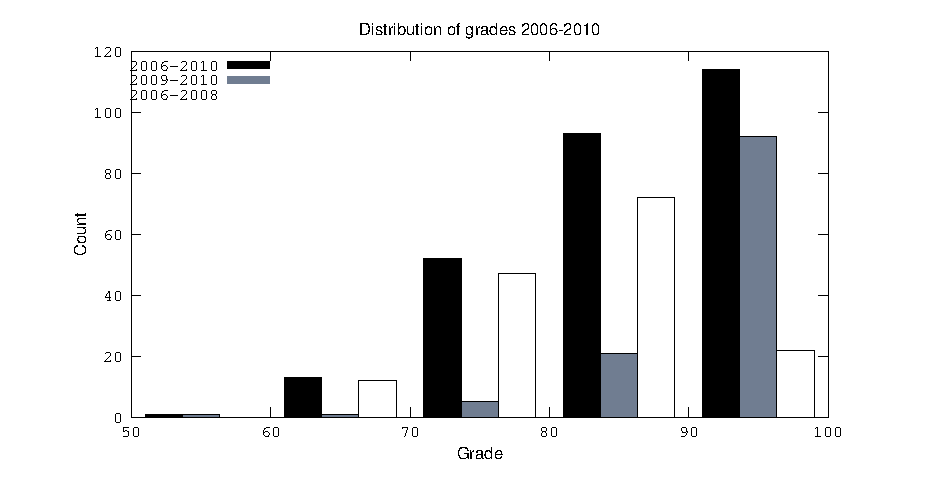
\includegraphics[width=0.8\linewidth]{526gradeDist}
\end{centering}

\section{Textbook}

There is no required textbook for this course, but buying one is
recommended.  

\textit{Optimization in economic theory} by \cite{dixit1990} is a very
readable. It lacks rigorous proofs, but does a great job of conveying
the intuition for results. It also contains many economic examples. 

The notes were originally largely based on \textit{Mathematics for
  Economists} by \cite{sb1994}. However, over time the content has
diverged somewhat. Nonetheless, Simon and Blume remains a good
reference. Compared to the notes, Simon and Blume place less emphasis
on proofs and more emphasis on examples and exercises. 

\textit{Fundamental Methods of Mathematical Economics} by
\cite{cw2005} is a good choice if you have little background in
mathematics and/or found the review exercises difficult. Chiang and
Wainwright is easier to read and has more economic motivation and
examples than Simon and Blume. However, Chiang and Wainwright does not
contain any proofs.

\textit{Foundations of Mathematical Economics} by \cite{carter2001} is
an excellent book, but is more difficult than the previous two. It
contains many proofs and can be quite abstract. However, it does do a
good job of motivating everything with economic examples. I recommend
it if you have a solid mathematics background or plan to continue
studying economics after the Master's program. 

All three books are available in affordable paperback
editions. Unfortunately, the UBC bookstore was unable to order
paperback editions, so you may want to order your book(s) elsewhere. 

\section{Course Outline}

This course has two main goals. One is to introduce some mathematical
techiniques that will be useful in other courses. The second is to
develop comfort with the sort of higher level mathematics that is used
throughout economics. The main mathematical technique that we will
focus on is optimization. Economics is largely about how to best
allocate scarce resources. Consumers maximize utlity subject to a
budget constraint, firms maximize profits subject to a production
possibilities constraint, and the social planner maximizers welfare
subject to a resource constraint. You are likely already familiar with
finite dimension constrained optimization. However, you might not
be familiar with optimization in infinite dimension. Infinite
dimensional optimization problems appear in economics when individuals
have to choose something at every instant of time or in every state of
the world. The first few weeks of the course will focus on solving
optimization problems, including those in inifinite dimension. 
After that, we will take a step back rigorously prove some of the
results that we have been using. In particular, we will cover some
basic real analysis and calculus on vector spaces. 

\begin{enumerate}
\item Optimization
  \begin{enumerate}
  \item Constrained optimization
  \item Comparative statics
  \item The maximum principle
  \item Dynamic programming
  \end{enumerate}
\item Sets and numbers
\item Linear algebra
  \begin{enumerate}
  \item Systems of linear equations 
  \item Matrix Algebra 
  \item Eigenvalues, eigenvectors, and definite matrices 
  \item Vector spaces
  \end{enumerate}
\item Calculus on vector spaces
  \begin{enumerate}
  \item Basic topology 
  \item Differential calculus 
  \item Inverse and implicit functions
  \item Optimization on vector spaces
  \end{enumerate}
\item Convexity and the separating hyperplane theorem
\item Comparative statics without differentiability: supermodularity
  and topkis's theorem 
\end{enumerate}
It is possible that we will not have time to cover all topics,
especially the last two.

\clearpage
\bibliographystyle{jpe}
\bibliography{../526}

\end{document}

